\documentclass{beamer}

\mode<presentation> {
  \usepackage{comment}
  \usepackage{pgfgantt}
  \usetheme{Madrid}
}

\usepackage{graphicx} 
\usepackage{booktabs} 
\usepackage{enumerate}
\usepackage{ragged2e}

\usepackage{geometry}
\usepackage{movie15}
\usepackage{hyperref}



%======================================================================================================
%======================================================================================================

\title[ProjectReview2]{Novel Video Analytics and Tapestry}
\logo{
\includegraphics[width=.8cm,keepaspectratio]{logo.png}}

\author[]{
  V. Alekhya
\newline
  Nadimpalli Vineetha
\newline
  Tarun Rajnish
\newline	
  Mohammed Talha Zubair
\newline
\newline
\small{
  Dr.Suryaprasad J
\newline  Batch No. 25}}

\institute[25]{}

\date[March 9, 2018]{March 9, 2018} 

%------------------------------------------------------------------------------------------------------

\begin{document}

%------------------------------------------------------------------------------------------------------
% SLIDE 1

\begin{frame}
  \titlepage 
\end{frame}

%------------------------------------------------------------------------------------------------------
% SLIDE 2

\section{Problem Statement}
\begin{frame}{Problem Statement}
To process the data obtained from CCTV footage via various static and dynamic video stitching techniques in order to detect intruder and display a time-line depicting the path traveled, computed from the feed of multiple cameras and do so in an optimized, efficient and simplified manner.
\end{frame}

%------------------------------------------------------------------------------------------------------
% SLIDE 3

\section{Block diagram}
\begin{frame}{High level block diagram}
  \begin{center}
    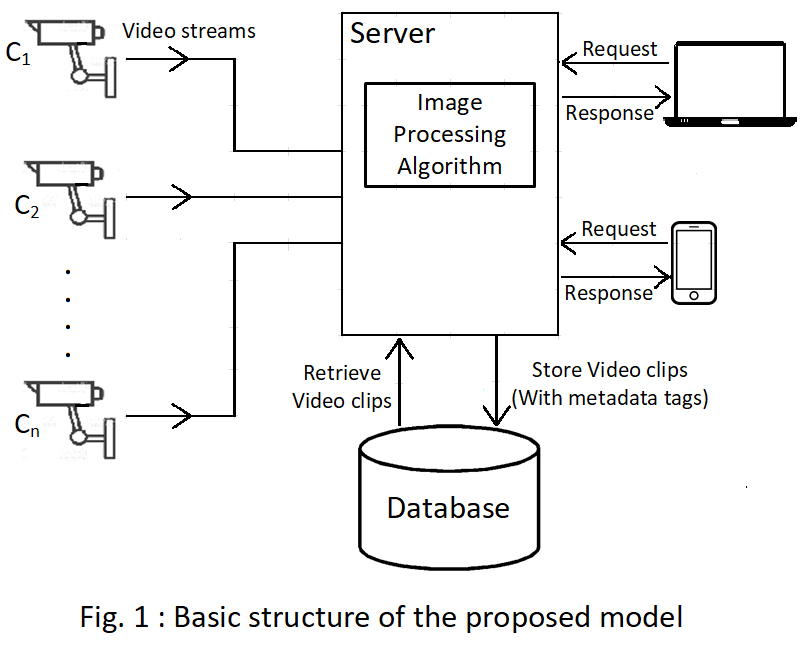
\includegraphics[width=10cm,keepaspectratio]{HighLevelBlockDiagram.png}
  \end{center}
\end{frame}

%------------------------------------------------------------------------------------------------------
% SLIDE 4

\section{System Requirements} 
\begin{frame}{System Requirements}
  \begin{itemize}
    \justifying  
    \item Language: Python 3 
    \newline
    \item Library: OpenCV
    \newline
    \item Operating System: Windows
    \newline

  \end{itemize}
\end{frame}

%------------------------------------------------------------------------------------------------------
% SLIDE 5

\section{Literature Survey} 
\begin{frame}{Literature Survey}
  \begin{itemize}
    %\justifying
    \item \textbf{A Context-Based Approach for Detecting Suspicious Behaviors}
    	  \newline 
          \textit{IEEE paper}
          \begin{itemize}
            \item Data stream model 
              \begin{itemize}
                \item Properties
                \item Advantages
              \end{itemize} 
            \item Single-pass algorithm vs Multi-pass algorithm
          \end{itemize}
  \end{itemize}
\end{frame}

%------------------------------------------------------------------------------------------------------
% SLIDE 6

\section{Literature Survey} 
\begin{frame}{Literature Survey}
  \begin{itemize}
    %\justifying          
    \item \textbf {Research and Design of the Intelligent Surveillance System Based on DirectShow and OpenCV}
          \newline 
          \textit{IEEE paper}
          \begin{itemize}
            \item Moving object detection methods
              \begin{itemize}
              \item Optical flow method
              \item Frame difference method
              \item Background subtraction method
              \end{itemize}
          \end{itemize}
   
  \end{itemize}
\end{frame}

%------------------------------------------------------------------------------------------------------
% SLIDE 7

\section{Block diagram}
\begin{frame}{Detailed Design}
  \begin{center}
    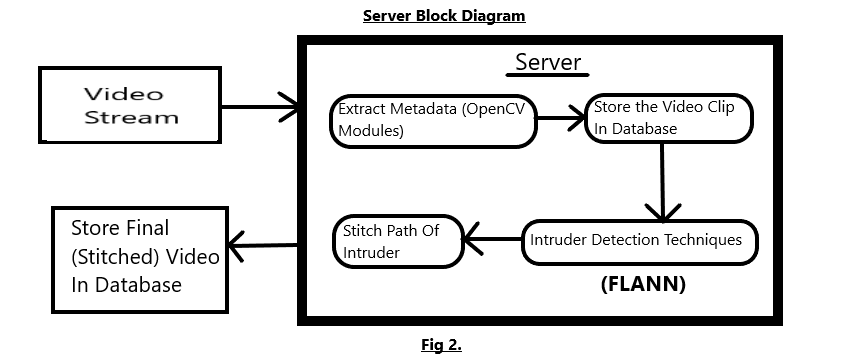
\includegraphics[width=10cm, height=10cm, keepaspectratio]{DetailedDesign1.png}
  \end{center}
\end{frame}

%------------------------------------------------------------------------------------------------------
% SLIDE 8

\section{Methodology} 
\begin{frame}{Methodology}
  \begin{itemize}
    %\justifying
   
    \item Extract feed with metadata from CCTV camera footage.
    \newline
    \item Use the below mentioned algorithms to find out intruder entry time compared to video time, track the intruder, etc. 
    \newline
    \item Capture snapshots (using multiple cameras) as the intruder moves through the campus and stitch together a tapestry of the trespassing path.
    \newline

  \end{itemize}
\end{frame}

%------------------------------------------------------------------------------------------------------
% SLIDE 9

\section{Implementation} 
\begin{frame}{Implementation}
  \begin{itemize}
    %\justifying
   
    \item Detect intruder (primary method)
    \newline
    \item Save video file and image of intruder
    \newline
    \item Check features of intruder with neighbouring videos and match
    \newline

  \end{itemize}
\end{frame}

%------------------------------------------------------------------------------------------------------
% SLIDE 10

\section{Intruder Detection Technique} 
\begin{frame}{Intruder Detection Technique}
  \begin{itemize}
    %\justifying
   
    \item Convert to gray scale and blur the frame
    \newline
    \item Compute absolute difference between first frame and current frame
    \newline
    \item Dilate the image and find contours
    \newline
    \item Compute bounding box for contours
    \newline

  \end{itemize}
\end{frame}

%------------------------------------------------------------------------------------------------------
% SLIDE 11

\section{Detection}
\begin{frame}{}
  \begin{center}
    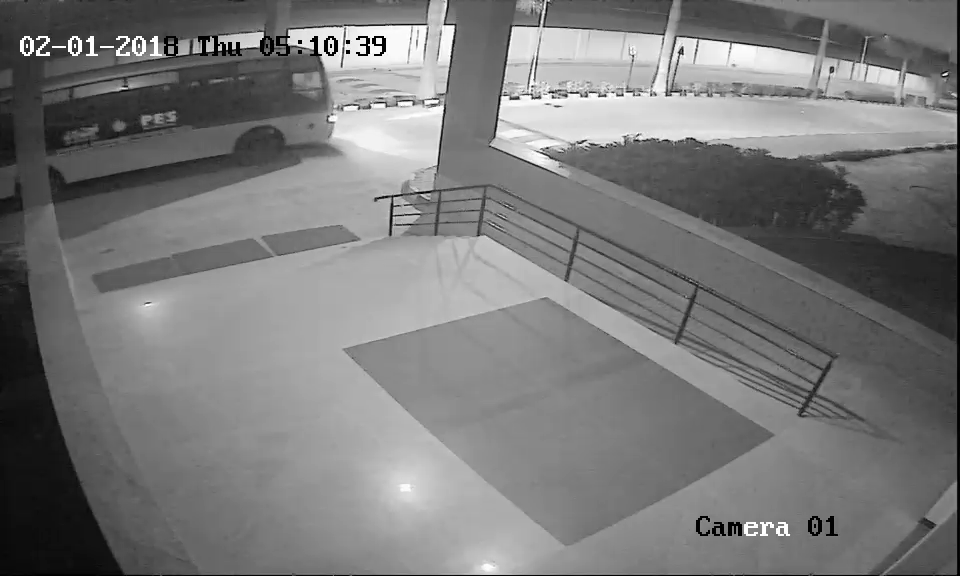
\includegraphics[width=10cm,keepaspectratio]{bus.png}
  \end{center}
\end{frame}

%------------------------------------------------------------------------------------------------------
% SLIDE 12

\section{Detection}
\begin{frame}{}
  \begin{center}
    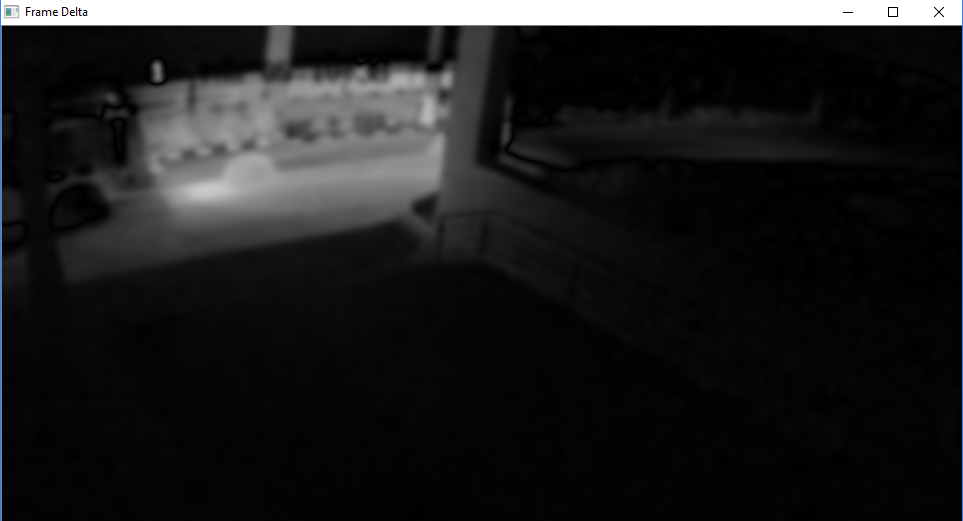
\includegraphics[width=6cm,keepaspectratio]{FrameDelta.png}
    \newline
    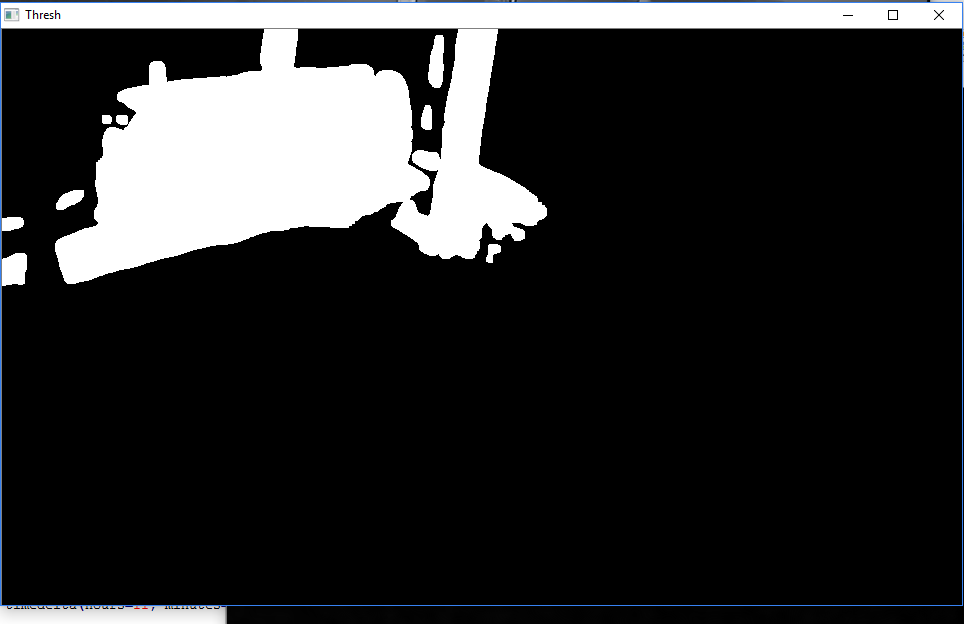
\includegraphics[width=6cm,keepaspectratio]{Grayscale.png}
  \end{center}
\end{frame}

%------------------------------------------------------------------------------------------------------
% SLIDE 13

\section{Detection}
\begin{frame}{}
  \begin{center}
    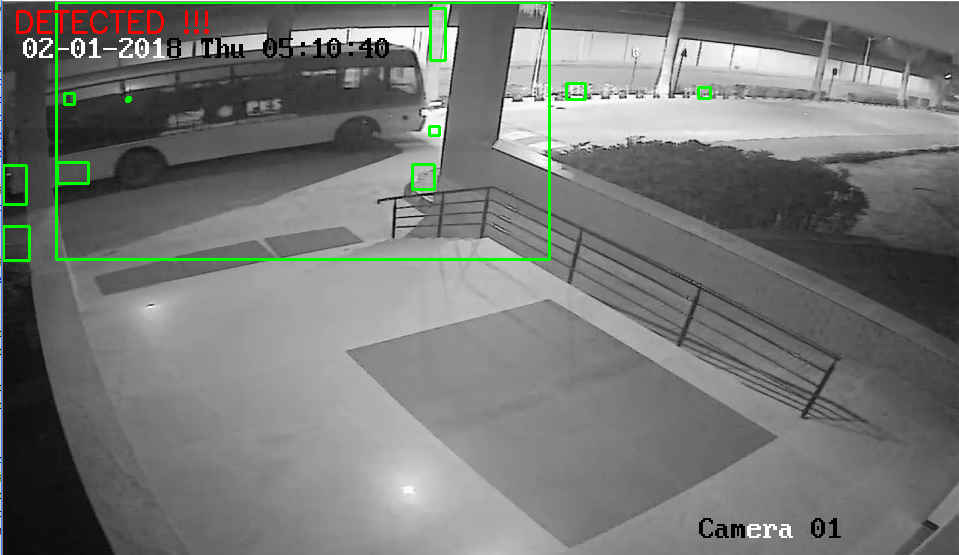
\includegraphics[width=10cm,keepaspectratio]{detection.png}
  \end{center}
\end{frame}


%------------------------------------------------------------------------------------------------------
% SLIDE 14

\section{Detection}
\begin{frame}{}
  \begin{center}
    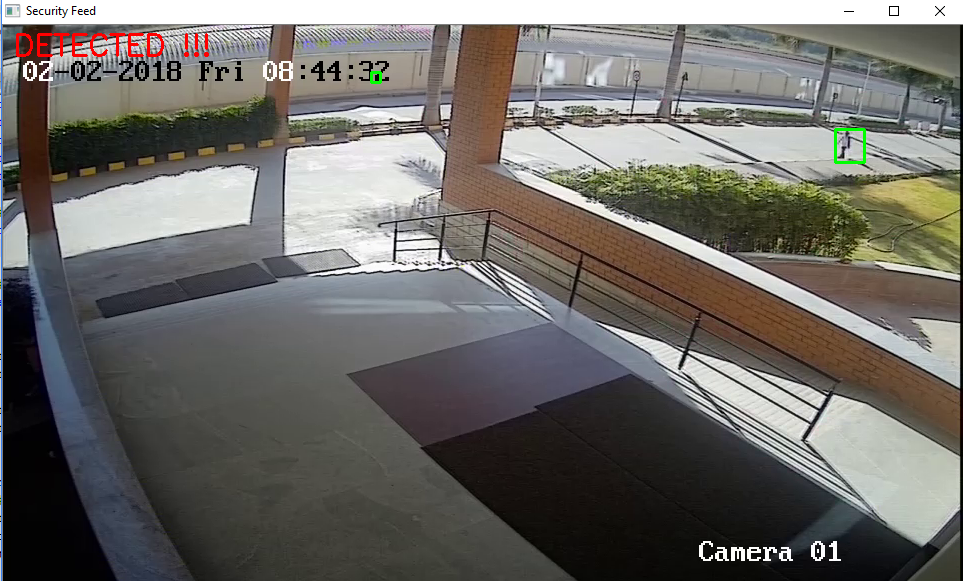
\includegraphics[width=10cm,keepaspectratio]{personDetection.png}
  \end{center}
\end{frame}

%------------------------------------------------------------------------------------------------------
% SLIDE 15

\section{Feature Detection Using FLANN} 
\begin{frame}{Feature Detection Using FLANN}
  \begin{itemize}
    %\justifying
   
    \item Fast Library for Approximate Nearest Neighbors
    \newline
    \item Optimized for fast nearest neighbor search in large datasets and for high dimensional features
    \newline
    \item Uses SIFT (Scale-Invariant Feature Transform)
    \newline
 

  \end{itemize}
\end{frame}

%------------------------------------------------------------------------------------------------------
% SLIDE 16

\section{Detection}
\begin{frame}{}
  \begin{center}
    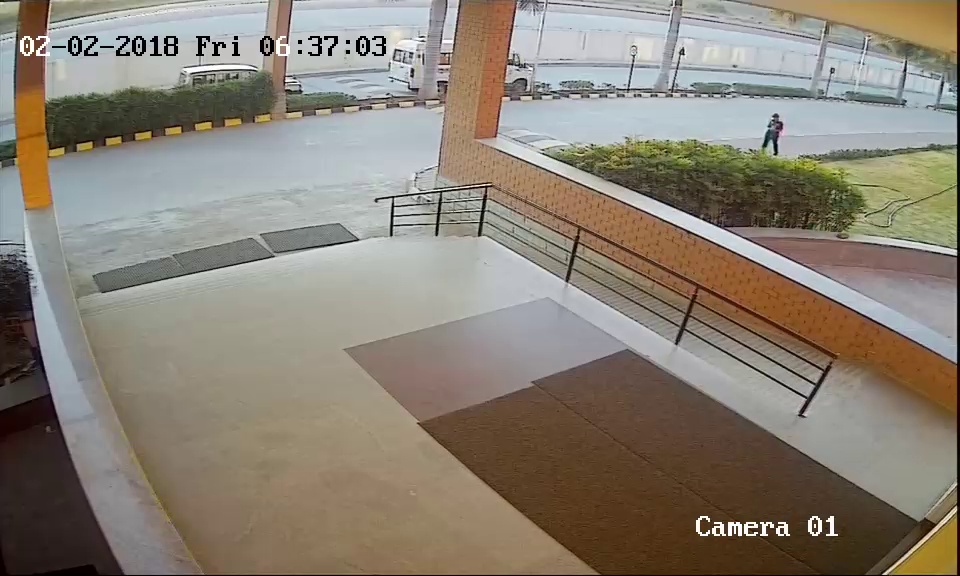
\includegraphics[width=8cm,keepaspectratio]{frame30.jpg}
    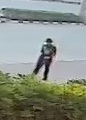
\includegraphics[width=3cm,keepaspectratio]{match.jpg}
  \end{center}
\end{frame}

%------------------------------------------------------------------------------------------------------
% SLIDE 17

\section{Detection}
\begin{frame}{}
  \begin{center}
    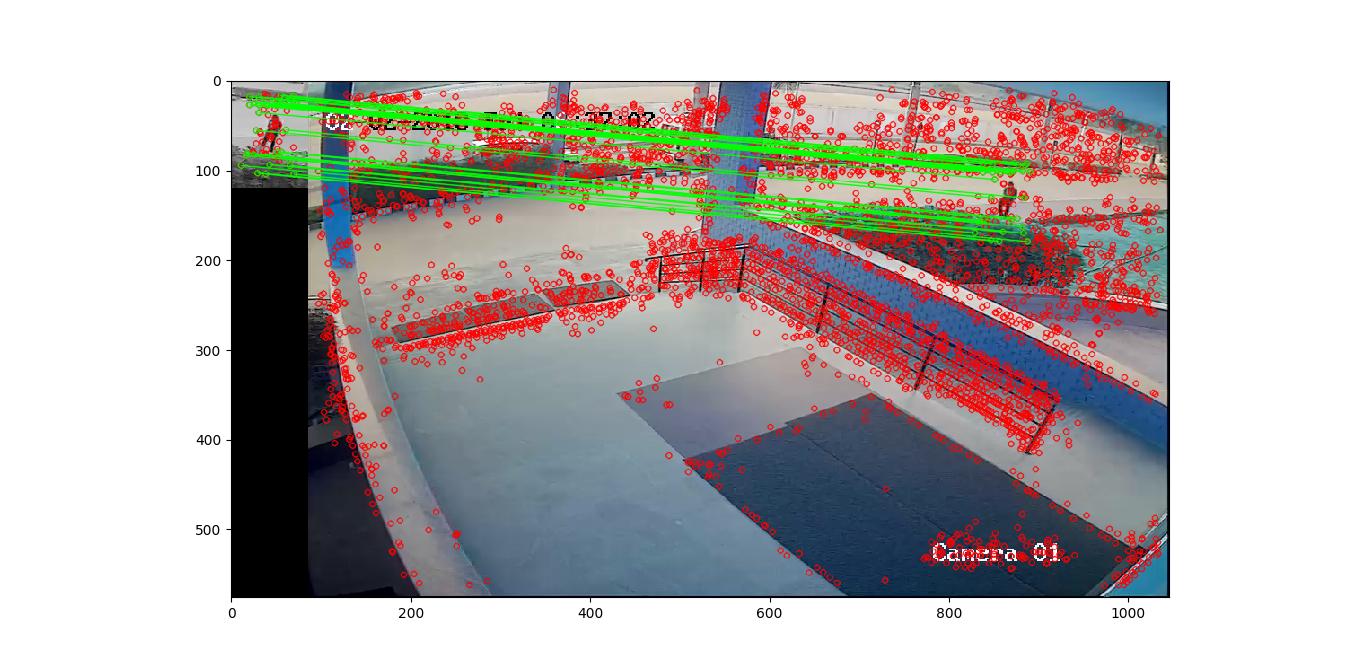
\includegraphics[width=13cm,keepaspectratio]{Figure_1.png}
  \end{center}
\end{frame}

%------------------------------------------------------------------------------------------------------
% SLIDE 18
\section{Detection}
\begin{frame}{}
  \begin{center}
    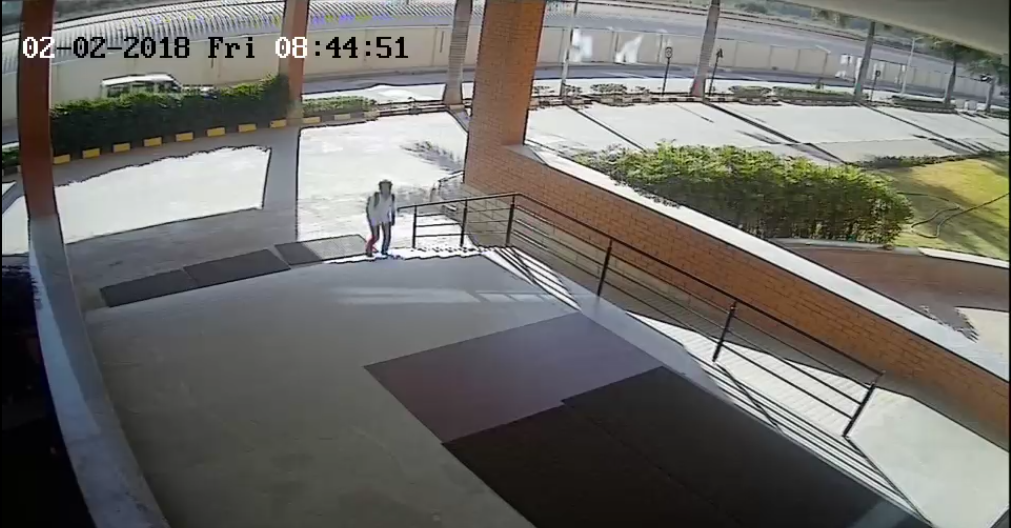
\includegraphics[width=7cm,keepaspectratio]{Untitled.png}
    \newline
     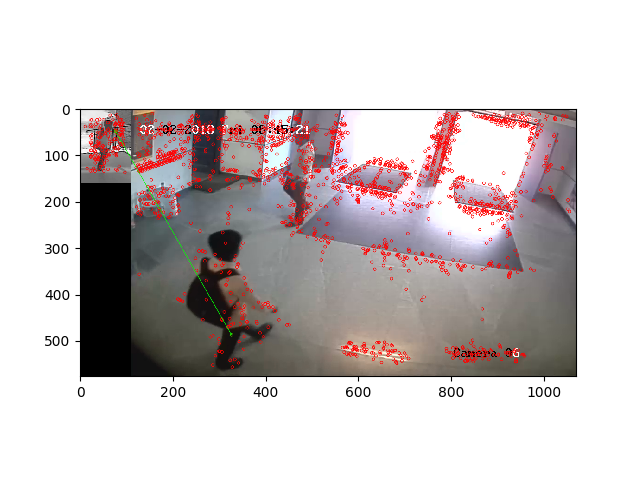
\includegraphics[width=8cm,keepaspectratio]{match.png}
  \end{center}
\end{frame}


%------------------------------------------------------------------------------------------------------
% SLIDE 19

\section{Next Steps} 
\begin{frame}{Next Steps}
  \begin{itemize}
    %\justifying
   
    \item Add secondary definitions for intruder
    \newline
    \item Add metadata tags and save 
    \newline
    \item Stitch video clips together based on tag
    \newline
    \item UI for video analytics
	\newline

  \end{itemize}
\end{frame}


%------------------------------------------------------------------------------------------------------
% SLIDE 20

\section{Schedule}
\begin{frame}
\frametitle{Time line of completion of project from Nov 2017-10th April 2018(Gantt Charts).}
\definecolor{barblue}{RGB}{153,204,254}
\definecolor{groupblue}{RGB}{51,102,254}
\definecolor{linkred}{RGB}{165,0,33}
\renewcommand\sfdefault{phv}
\renewcommand\mddefault{mc}
\renewcommand\bfdefault{bc}
\setganttlinklabel{s-s}{START-TO-START}
\setganttlinklabel{f-s}{FINISH-TO-START}
\setganttlinklabel{f-f}{FINISH-TO-FINISH}
\sffamily
\begin{ganttchart}[
    canvas/.append style={fill=none, draw=black!5, line width=.75pt},
    hgrid style/.style={draw=black!5, line width=.75pt},
    vgrid={*1{draw=black!5, line width=.75pt}},
    today=7,
    today rule/.style={
      draw=black!64,
      dash pattern=on 3.5pt off 4.5pt,
      line width=1.5pt
    },
    today label font=\small\bfseries,
    title/.style={draw=none, fill=none},
    title label font=\bfseries\footnotesize,
    title label node/.append style={below=7pt},
    include title in canvas=false,
    bar label font=\mdseries\small\color{black!70},
    bar label node/.append style={left=2cm},
    bar/.append style={draw=none, fill=black!63},
    bar incomplete/.append style={fill=barblue},
    bar progress label font=\mdseries\footnotesize\color{black!70},
    group incomplete/.append style={fill=groupblue},
    group left shift=0,
    group right shift=0,
    group height=.5,
    group peaks tip position=0,
    group label node/.append style={left=.6cm},
    group progress label font=\bfseries\small,
    link/.style={-latex, line width=1.5pt, linkred},
    link label font=\scriptsize\bfseries,
    link label node/.append style={below left=-2pt and 0pt}
  ]{1}{13}
  \gantttitle[
    title label node/.append style={below left=7pt and -3pt}
  ]{WEEKS:\quad1}{1}
  \gantttitlelist{2,...,13}{1} \\
  \ganttgroup[progress=52]{Summary Element 1}{1}{10} \\
  \ganttbar[
    progress=85,
    name=WBS1A
  ]{\textbf{1} Problem Statement,Survey}{1}{3} \\
  \ganttbar[
    progress=70,
    name=WBS1B
  ]{\textbf{2} Requirements Specification}{3}{5} \\
  \ganttbar[
    progress=50,
    name=WBS1C
  ]{\textbf{3}Intrusion and Tapestry}{5}{11} \\
  \ganttbar[
    progress=0,
    name=WBS1D
  ]{\textbf{4} Analytics and Final Testing}{11}{15} \\[grid]
  
\end{ganttchart}

%\begin{columns}[c] % The "c" option specifies centered vertical alignment while the "t" option is used for top vertical alignment

%\column{.45\textwidth} % Left column and width
%\textbf{Heading}
%\begin{enumerate}
%\item Statement
%\item Explanation
%\item Example
%\end{enumerate}

%\column{.5\textwidth} % Right column and width
%Lorem ipsum dolor sit amet, consectetur adipiscing elit. Integer lectus nisl, ultricies in feugiat rutrum, porttitor sit amet augue. Aliquam ut tortor mauris. Sed volutpat ante purus, quis accumsan dolor.

%\end{columns}
\end{frame}

%------------------------------------------------------------------------------------------------------
% SLIDE 21

\section{References}
\begin{frame}{References}
  \footnotesize{
  \begin{thebibliography}{99}
    \bibitem{p1} Arnold Wiliem, Vamsi Madasu, Wageeh Boles, and Prasad Yarlagadda
    \newblock A Context-Based Approach for Detecting Suspicious Behaviors
    \newblock \emph{IEEE, 2009}

    \bibitem{p1} Chaoyu Lin , Yuliang Tang
    \newblock Research and Design of the Intelligent Surveillance System Based on DirectShow and OpenCV
    \newblock \emph{IEEE, 2011}

    \bibitem{p1} B. Cotton
    \newblock Enhancing a city’s ability to plan, protect and manage with intelligent video analytics, 				  Tech. Rep. 
    \newblock GPW12348-USEN-00 
    \newblock \emph{A Frost \& Sullivan White paper}
  \end{thebibliography}
  }
\end{frame}

%------------------------------------------------------------------------------------------------------
% SLIDE 22

\section{References}
\begin{frame}{References}
  \footnotesize{
  \begin{thebibliography}{99}
    \bibitem{p1} James  M. Ferryman, Andrew A. Adams
    \newblock The future of video analytics for surveillance and its ethical implications
    \newblock \emph{Security Journal, 2012}

    \bibitem{p1} AGENT VI
    \newblock White paper agent video intelligence tech. rep.,
    \newblock \emph{JULY 2016}

  \end{thebibliography}
  }
\end{frame}

%------------------------------------------------------------------------------------------------------
% SLIDE 23

\begin{frame}
\textcolor{blue}{\Huge{\centerline{The End}}}
\end{frame}

%------------------------------------------------------------------------------------------------------

\end{document}

%======================================================================================================
%======================================================================================================
